% This is samplepaper.tex, a sample chapter demonstrating the
% LLNCS macro package for Springer Computer Science proceedings;
% Version 2.20 of 2017/10/04
%
\documentclass[runningheads]{llncs}
%
\usepackage{pgfgantt}

\usepackage{graphicx}
\usepackage[strings]{underscore}
\usepackage[hyphens]{url}
\usepackage{ragged2e}
\usepackage{tabularx}
\usepackage[ruled,vlined]{algorithm2e}
\usepackage{listings}
\usepackage{caption}
\usepackage{subcaption}
\usepackage{layouts}

% set custom section numbers depth
\setcounter{secnumdepth}{5}
\usepackage{listings}
\usepackage{xcolor}
\usepackage{amsmath}

% define styling for code highlighting
\definecolor{codegreen}{rgb}{0,0.6,0}
\definecolor{codegray}{rgb}{0.5,0.5,0.5}
\definecolor{codepurple}{rgb}{0.58,0,0.82}
\definecolor{backcolour}{rgb}{0.95,0.95,0.92}

\lstdefinestyle{mystyle}{
	backgroundcolor=\color{backcolour},   
	commentstyle=\color{codegreen},
	keywordstyle=\color{magenta},
	numberstyle=\tiny\color{codegray},
	stringstyle=\color{codepurple},
	basicstyle=\ttfamily\footnotesize,
	breakatwhitespace=false,         
	breaklines=true,                 
	captionpos=b,                    
	keepspaces=true,                 
	numbers=left,                    
	numbersep=5pt,                  
	showspaces=false,                
	showstringspaces=false,
	showtabs=false,                  
	tabsize=2,
	frame=single
}
\lstset{style=mystyle}

\setlength{\parindent}{0in}
% Used for displaying a sample figure. If possible, figure files should
% be included in EPS format.
%
% If you use the hyperref package, please uncomment the following line
% to display URLs in blue roman font according to Springer's eBook style:
% \renewcommand\UrlFont{\color{blue}\rmfamily}
\renewcommand\refname{Literaturangaben}

\begin{document}
%
\title{Hauptprojekt \\~\\ Konzeption und prototypische Implementierung einer verteilten Autoscaling-Architektur für Cloud-Bursting mit Container-as-a-Service}
%
\titlerunning{Hauptprojekt}
% If the paper title is too long for the running head, you can set
% an abbreviated paper title here
%
\author{Christian F. Bargmann}
%
% \authorrunning{F. Author et al.}
% First names are abbreviated in the running head.
% If there are more than two authors, 'et al.' is used.
%
\institute{Hamburg University of Applied Sciences, Berliner Tor 5, 20099 Hamburg, Germany \\
	\email{christian.bargmann@haw-hamburg.de} \\
	\url{https://www.haw-hamburg.de}}
%
\maketitle              % typeset the header of the contribution
%
\begin{abstract} Der Begriff Cloud-Bursting ist in den letzten Jahren populär geworden. Hierbei wird eine Anwendung in einer privaten Cloudumgebung oder einem Rechenzentrum betrieben. Steigt die Nachfrage an Rechenkapazität an, werden automatisch Ressourcen in einer öffentlichen Cloud provisioniert. Die Entscheidung, anhand welcher Kriterien Res\-sourcen in eine öffentliche Cloud ausgelagert werden, wie sich die provisonierten Ressourcen in die lokal betriebene Infrastruktur integrieren lassen und welches Servicemodell des Cloud-Providers verwendet werden soll, ist in den vergangenen Jahren in den Fokus aktueller Forschung gerückt. Dieses Hauptprojekt konzeptioniert, implementiert und evaluiert eine verteilte Autoscaling-Architektur für Cloud-Bursting in Hybrid-Clouds, die automatisiert Ress\-ourcen auf Basis von Metriken als Container-as-a-Service bei mehreren Cloud-Service-Providern provisionieren und skalieren kann.
		
	\keywords{Cloud Bursting \and Cloud Computing \and Autoscaling \and \newline Container \and Software Architektur}
\end{abstract}
%
%
%
	
\section{Einleitung} \label{motivation}
	
Cloud-Bursting ist ein Betriebsmodell, bei dem eine Anwendung in einer privaten Cloudumgebung oder einem Rechenzentrum betrieben wird, jedoch automatisch Ressourcen einer öffentlichen Cloud provisioniert werden, wenn die Nachfrage nach Rechenkapazität ansteigt. Bei diesem hybriden Betriebsmodell wird die eigene Infrastruktur vollständig genutzt, so dass eine Anzahl von Servern in eigener Verantwortung und Kontrolle betrieben werden kann. Gleichzeitig besteht bei Lastspitzen die Möglichkeit, die Anwendung ganz oder teilweise in eine externe, öffentliche Cloud zu verlagern. \\
	
Die wichtigste Technologie bei Cloud-Computing zum Hosten und Verwalten von Anwendungen ist die Virtualisierung. Traditionell wird Hardware-Level-Virtualisierung, auch bekannt als Hypervisor-basierte Virtualisierung, zur Verwaltung von virtuellen Maschinen (VMs) in Cloud-Rechenzentren verwendet. Ein großer Fortschritt in der Virtualisierungstechnologie ist die Containerisierung von Anwendungen, die auch als Virtualisierung auf Betriebssystemebene bekannt ist. Aufgrund der besseren Portabilität, des geringen Ressourcenbedarfs und der einfachen Skalierbarkeit im Vergleich zur VM-basierten Virtualisierung, hat Containerisierung in den letzten Jahren deutlich an Popularität gewonnen. Containerisierung eignet sich für die Verwaltung von Microservices, da sie das schnelle Starten und Beenden von Containern und somit schnelle Skalierbarkeit unterstützt, während die VM-basierte Virtualisierung vergleichsweise mehr Zeit für das Starten und Beenden der VM benötigt \cite{al-dhuraibi_elasticity_2018}, \cite{abdullah_containers_2019}. Viele Cloud-Service-Provider (CSPs) bieten Container-as-a-Service Angebote an, mit denen sich Container in einer Cloud-Umgebung betreiben lassen, ohne die darunterliegende Infrastruktur selbst verwalten zu müssen. \\

Für viele Unternhemen ist es unterschiedlichsten Gründen nicht möglich, ihre gesamte Infrastruktur zu einen CSP zu verlagern. Trotzdem bietet es sich situationsbedingt an, Teile der Infrastruktur bei Lastspitzen auszulagern und kurzzeitig die eigenen Rechenkapazitäten durch das Hinzuziehen von Ressourcen eines CSP zu steigern.
Trotz moderner As-a-Service-Angebote, ist die Umsetzung eines Hybrid-Cloud-Ansatzes für viele Unternehmen ein nicht zu unterschätzender Aufwand. Die Integration zwischen der eigenen Infrastruktur und den Schnitt\-stellen der CSPs, sowie die Wahl von geeigneten Skalierungsmethoden, ohne dabei zu stark an eine bestimmte Cloud-Plattform gekoppelt zu sein, ist dabei eine große Herausforderung.  \\

In dieser Arbeit wird eine verteilte Autoscaling-Architektur für Cloud-Bursting in Hybrid-Clouds vorgestellt, die automatisiert Ressourcen auf Basis von Metriken als Container-as-a-Service bei einem CSP provisionieren und horizontal skalieren kann. Die vorgestellte Architektur ist in der Lage, Anwendungen über mehrere Cloud-Umgebungen hinweg zu skalieren und provisionierte Ressourcen von meh\-reren Anbietern parallel in die eigene lokale Infrastruktur einzubinden. Für die automatische Skalierung von internen Ressourcen bei Lastspitzen zu CSPs werden Metriken aus externen Monitoring-Systemen genutzt, statt eigene Metriken zu implementieren. Im Vergleich zu anderen Ansätzen (vgl. Abschnitt \ref{work}.), setzt die hier präsentierte Lösung nicht voraus, das lokal ein Container-Cluster betrieben wird, was den Einsatz dieser Lösung attraktiv für Anwender macht, die kein Container-Cluster betreiben können, aber trotzdem ein Autoscaling für lokal betriebene Anwendungen benötigen. Auch müssen lokal betriebene Anwendungen nicht modifiziert werden, um durch die vorgestellte Architektur skaliert zu werden. Die Komponenten der Autoscaling-Architektur können sowohl On-Premise, als auch extern bei einem CSP betrieben werden. \\

Desweiteren wird ein Prototyp mit einer reaktiven Skalierungstechnik, die den Lebenszyklus von Ressourcen berücksichtigt, implementiert und das Verhalten der Autoscaling-Architektur unter verschiedenen Lastszenarien evaluiert.

	
\section{Related Work} \label{work}

In Folgendem Abschnitt werden Arbeiten präsentiert, die eine Architektur für das automatische Skalieren von Ressourcen vorstellen. Die Auswahl ist dabei nicht auf Architekturen mit Multi-Provider Fähigkeit beschränkt. Desweiteren werden aktuelle Skalierungstechniken erläutert. 
	
\subsection{Autoscaling-Architekturen}

Danayi et al. \cite{danayi_opencot_2019} präsentieren in ihrer Arbeit eine Implementierung eines Cloud Managers für das Internet of Things. Die vorgestellte Architektur nutzt Function-as-a-Service (FaaS) als Servicemodell, um bei Lastspitzen einzelne Funktionen zu einem öffentlichen Cloud-Provider auszulagern. Hierbei wird ein zentraler Cloud-Broker als Gateway-Komponente verwendet, der sämtliche Funktionsanfragen entgegennimmt und Logik zur Skalierung von Ressourcen an eine Controller-Komponente delegiert. Das Framework nutzt und speichert eigene Metriken für die Skalierung von Ressourcen und ist auf die Programmiersprache Python beschränkt. Für das Internet of Things bietet sich FaaS als ein geeignetes Servicemodell an, jedoch kann FaaS für viele Anwendungszenarien zu feingranular sein. \\
	
Biswas et al. \cite{biswas_auto-scaling_2015} erläutern ein Framework mit einer reaktiven Skalierungsmethode, um Service-Level-Objective (SLO)-basierte und nicht SLO-basierte Anfragen zu verarbeiten. In einer fortführenden Arbeit werden hybride Skalierungsmethoden anhand von Kostenanalysen präsentiert \cite{biswas_hybrid_2017}. Hierbei wird der Cloud Broker bei einem Drittunternehmen eingesetzt, welches im Bedarfsfall Ressourcen für die private Cloud des Klienten bei einem Public-Cloud-Anbieter provisioniert. Der Klient hat keine Kontrolle über den eingesetzten Broker des Drittunternehmens, ebenso ist der Broker stark gekoppelt an die Schnittstellen des Public-Cloud-Providers. \\
	
Ye et al. \cite{ye_auto-scaling_2017} stellen eine Autoscaler-Architektur mit hybriden Skalierungsmethoden vor, die in einer containerbasierten, privaten Cloudumgebung eingesetzt werden können und sowohl das aktuelle Anfragevolumen, als auch SLOs für die geeignete Skalierung von Ressourcen berücksichtigen. Zwar werden hier automatisch Ressourcen bei Lastspitzen in der eigenen private Cloudumgebung skaliert, allerdings werden  keine externen Ressourcen hinzugezogen. \\

Gandhi et al. \cite{gandhi_adaptive_nodate} präsentieren in ihrer Arbeit eine Architektur für einen voll\-ständig automatisierten Cloud-Service, der proaktiv deployte Anwendungen in einer Cloud-Infrastruktur auf Basis einer Kombination aus anwendungs- und systemspezifischen Metriken skalieren kann. Als zu skalierende Instanzen werden keine Container, sondern virtuelle Maschinen verwendet. Die Architektur ist in der Lage, über die Schnittstellen der Cloud-Infrastruktur dynamisch VMs zu provisionieren und einzubinden, sowie Ressourcenkapazitäten anzupassen. Um ein Autoscaling der lokalen Infrastruktur durchzuführen, ist der Einsatz von on-premise Cloud-Infrastruktur und IaaS-Diensten notwendig. \\
	
Chandra \cite{chandra_cloud_2020} stellt eine Möglichkeit für Cloud-Bursting mithilfe der Kubernetes-Erweiterungen Virtual Kubelet\footnote{https://github.com/virtual-kubelet/virtual-kubelet} und KIP\footnote{https://github.com/elotl/kip} vor. Die vorgestellte Methode setzt den Betrieb eines eigenen Clusters in der privaten Cloudumgebung voraus und nutzt Autoscaling-Funktionalitäten des Container-Orchestrators Kubernetes für die horizontale Skalierung von Container-Instanzen. Es wird vorausgesetzt, dass die zu skalierenden Instanzen zuvor als ein Deployment im Cluster angelegt worden sind. Weiterhin beschreibt Mennig \cite{mennig_cloud_2020} einen Multicluster-Ansatz mit dem Einsatz von Service Meshes, um Cloud Bursting umzusetzen. Hier wird Cluster-as-a-Service als Servicemodell beim Public-Cloud-Provider genutzt, um Compute Cluster zu provisionieren und diese in die on-premise betriebene Cluster-Infrastruktur einzubinden. Ein Service-Mesh wird für die Cross-Cluster-Kommu\-nikation von Ressourcen verwendet, gemeinsam mit einem Multicloud-Scheduler um Workloads bei Lastspitzen über mehrere Cluster zu verteilen. Auch hier wird jedoch der Betrieb einer eigenen Cloud-Infrastruktur vorausgesetzt, ebenso wird Expertenwissen benötigt für die Installation und Wartung der Cluster-Erweiterungen, was für viele Unternehmen ein nicht zu unterschätzender Aufwand ist.
	
\subsection{Provisionierung von Ressourcen}

In verteilten Umgebungen wie Clouds, ist eine geeignete Skalierung von Ressourcen wichtig. Eine Unterskalierung kann zu hohen Antwortzeiten oder einer großen Anzahl abgelehnter Anfragen führen.  Eine Überskalierung wiederum verursacht nicht ausgelastete Ressourcen, wodurch Zusatzkosten für ungenutzte Rechenleistung entstehen. \\

Die Entscheidung über die Allokierung oder Freigabe von Ressourcen in Clouds, basiert in der Regel auf überwachten oder vorhergesagten Low-Level-Performance-Indikatoren (z.B. Auslastung von Ressourcen wie CPU, Speicher, Netzwerkbandbreite) oder High-Level-Indikatoren (z.B. Antwortzeit, Anfragerate). Weitere Metriken um ein Quality of Service (QoS) zu gewährleisten, werden auch in [17] und [18] vorgeschlagen. Zusammenfassend ist das Ziel dieser Arbeiten, bestimmte Werte von überwachten Indikatoren innerhalb  festgelegter Thresholds zu halten und bei Abweichung Skalierungsmechanismen auszulösen. Eine automatische Skalierung von Ressourcen kann reaktiv durchgeführt werden, zum Beispiel als Folge von Änderungen der Arbeitslast, oder proaktiv, d.h. anhand Vorhersagen von Änderungen der Arbeitslast. In mehreren Arbeiten werden auch Kombinationen der beiden Ansätze vorgeschlagen \cite{ali-eldin_adaptive_2012}, \cite{gandhi_adaptive_nodate}, \cite{fernandez_autoscaling_2014}, \cite{bouabdallah_use_2016}. Desweiteren gibt es Arbeiten wie \cite{moreno-vozmediano_efficient_2019}, \cite{iqbal_unsupervised_2016} und \cite{bu_reinforcement_2009}, in denen maschinelles Lernen und analytische Verfahren für eine prädiktive Autoskalierung vorgestellt werden. \\

In dieser Arbeit wird eine reaktive Skalierungsstrategie vorgestellt, implementiert und in Abschnitt \ref{skalierungstechnik} im Detail erläutert. Verwendet werden vom Administrator festgelegte Regeln in Form von SLOs zur Einaltung bestimmter Thresholds.  \\
	
\section{Architekturübersicht} \label{Architekturübersicht}
	
In diesem Abschnitt wird auf die entwickelte Autoscaler-Architektur beschrieben. Zunächst wird ein Überblick über den Anwendungskontext gegeben und das Datenmodell vorgestellt. Anschließend wird auf die einzelnen Komponenten der Architektur im Detail eingegangen und die Skalierungstechnik für die Allokierung und Freigabe von Ressourcen erläutert.
	
\subsection{Architektur}

Die Systemarchitekur des verteilten Autoscalers für Cloud-Bursting in Hybrid-Clouds ist in Fig. \ref{systemarchitektur} dargestellt. Abgebildet sind sowohl die interne on-premise, als auch externe Infrastruktur des CSPs. Der Autoscaler selbst besteht auf mehreren Teilanwendungen, die jeweils in einem eigenen Prozess gestartet werden und gemeinsam die automatische Skalierung von lokalen Anwendungen umsetzen.
	
\begin{figure}
	\centering
	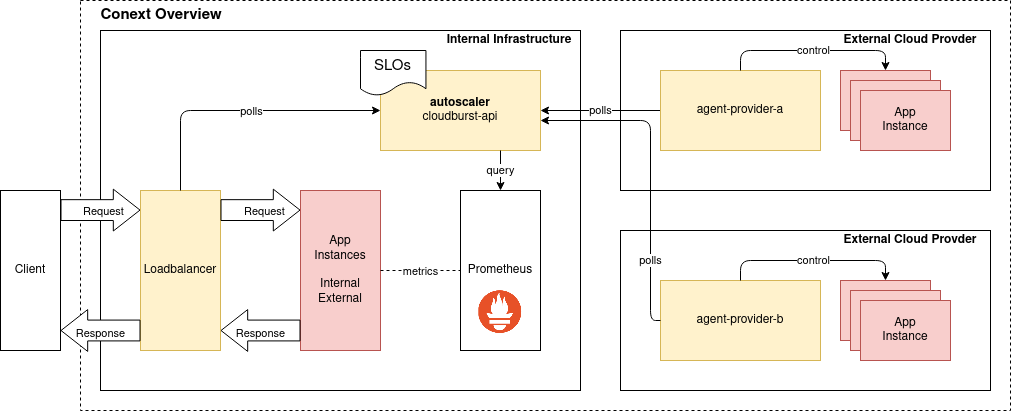
\includegraphics[width=1.0\linewidth,scale=1.0]{images/context.png}
	\caption{Systemarchitektur und Kontextdarstellung der Autoscaling-Architektur}
	\label{systemarchitektur}
\end{figure}

Voraussetzung für das automatische Skalieren einer lokal bereitgestellten Anwendung ist, dass diese Metriken zur Laufzeit exportiert und durch ein Monitoring-Tool überwacht wird. Außerdem muss die zu skalierende Anwendung oder ein deploybarer Teil der Anwendung als ausführbarer Container in einer Container-Registry vorliegen. \\

Kernelement der Architektur ist die Control-Plane-Komponente (vgl. \ref{control_plane}), welche in regelmäßigen Intervallen die von einem Administrator festgelegten SLOs gegen\-über dem Monitoring-Tool evaluiert und die Allokierung oder Freigabe von Ressourcen berechnet. Über eine Webschnittstelle rufen die Agent-Komponenten über ein Polling-Ansatz regelmäßig den Status über zu startende oder zu terminierende Instanzen zu einem Zeitpunkt ab. Im Vergleich zur Control-Plane sind die Agents statuslos und setzen den durch den Autoscaler berechneten Bedarf an Instanzen zu einem Zeitpunkt bei einem CSP um. \\

Für jeden CSP zu dem Instanzen bei einer automatischen Skalierung ausgelagert werden sollen, wird genau ein Agent deployed. Weitere CSPs können über die Implementierung eines Interfaces angebunden werden. Bei jeder Statusveränderung einer Instanz (vgl. Status) schreibt der Agent diese zurück an die Control-Plane. Zwischen dem aufrufenden Client und der zu skalierenden Anwendung ist ein Proxy geschaltet, der als Loadbalancer agiert. Der Proxy nutzt ebenfalls einen Polling-Ansatz um die Routeninformationen von gestarteten Instanzen bei den CSPs zu erfragen. Anfragen, die den Proxy durchlaufen, werden nun automatisch zwischen lokalen und externen Instanzen einer Anwendung geroutet.

\subsection{Datenmodell}

\begin{figure}
	\centering
	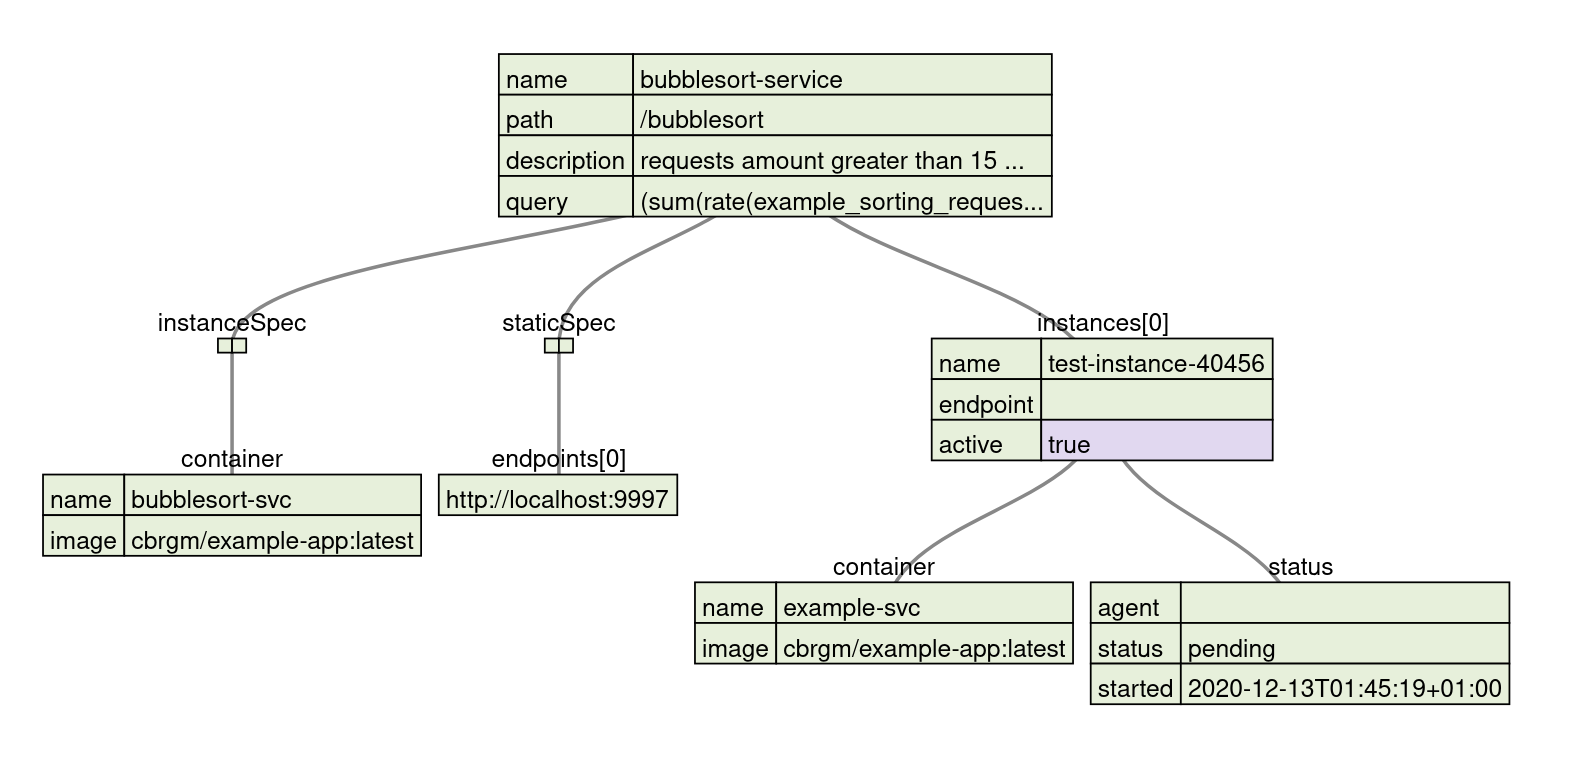
\includegraphics[width=0.8\linewidth,scale=0.8]{images/datamodel.png}
	\caption{Entitäten der Autoscaling-Architektur, dargestellt als Baumdiagramm}
	\label{datenmodell}
\end{figure}

Die Entitäten sind in Fig. \ref{datenmodell} dargestellt. Eine Anwendung besteht aus mehreren Services, wobei ein Service das Element einer automatischen Skalierung durch den Autoscaler sein soll. Diese Services werden in einer Konfigurationsdatei (vgl. \ref{configuration}) als sogenannte \textit{ScrapeTargets} definiert. Ein ScrapeTarget beschreibt einen Service mit einer Metrikabfrage, die in Intervallen an das Monitoring-Tool gesendet und für die Berechnung der Skalierung eines Services evaluiert wird. Auch wird beschrieben, wie die zu startende Container-Instanz bei einem CSP parametrisiert (\textit{InstanceSpec}) wird und welche Instanzen in der lokalen Infrastruktur ausgeführt werden (\textit{staticSpec}). \\

Einem Service (\textit{ScrapeTarget}) sind mehrere Instanzen (\textit{Instances}) zugeordnet. Eine Instanz beschreibt einen zustandsbehafteten Prozess, in dem die zu skalierende Anwendung oder Teilanwendung ausgeführt wird oder ausgeführt werden soll. Die Parameterbeschreibung eines Containers  in einem ScrapeTarget dient als Schablone für das Erstellen von Instanzen, die einem Service zugeordnet sind.

\begin{figure}
	\centering
	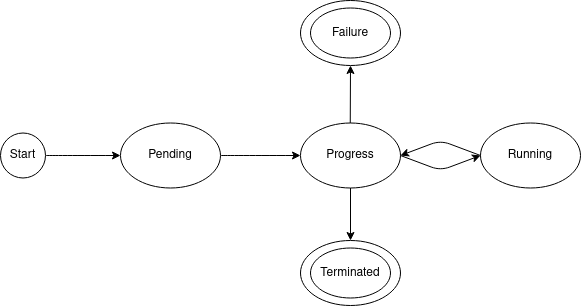
\includegraphics[width=0.6\linewidth,scale=0.6]{images/state.png}
	\caption{Zustandsdiagramm für Instanzen}
\end{figure}

Instanzen besitzen einen Lebenszyklus, welcher durch die Bearbeitung durch die Agent-Komponente verändert wird. Diese Statusveränderungen werden als \textit{Status} in einer Instanz vermerkt.
	
\subsection{Control Plane} \label{control_plane}

Die Control-Plane ist das Kernelement der Autoscaling-Architektur. Für jeden zu skalierenden Service, wird in zeitlichen Intervallen die festgelegte Metrik von dem Monitoring-Tool abgefragt. Das Ergebnis dieser Abfrage wird in die Berechnung für den Bedarf neuer Instanzen einkalkuliert. Anhand des Bedarfes wird der Zustand der Control-Plane modifiziert. Über eine RESTful Webschnittstelle können andere Komponenten wie der Proxy und die Agents diesen Zustand abrufen und verändern, beispielsweise wenn der Status einer Instanz aktualisiert wurde. \\

\begin{figure}
	\centering
	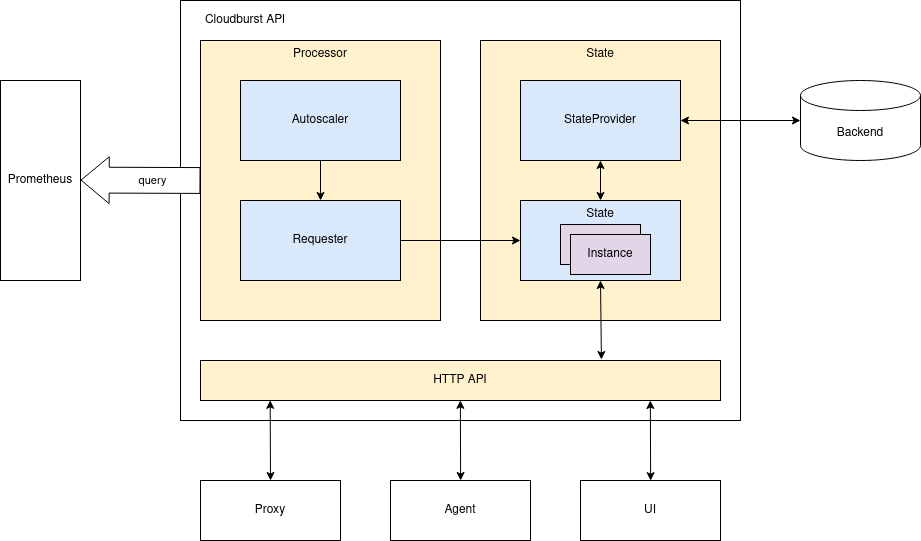
\includegraphics[width=0.8\linewidth,scale=0.8]{images/autoscaler.png}
	\caption{Komponentendiagramm der Control-Plane Komponente}
\end{figure}

In der hier vorgestellten Implementierung wird Prometheus\footnote{https://github.com/prometheus} als Monitoring-Tool verwendet.  Prometheus zeichnet Echtzeitmetriken in einer Zeitreihendatenbank auf, die über Webaufrufe von Anwendungenen abgefragt werden. Außerdem bietet Prometheus eine funktionale Abfragesprache namens \textit{PromQL} (Prometheus Query Language) an, mit der Clients Zeitreihendaten in Echtzeit selektieren und aggregieren können. Das Ergebnis eines Ausdrucks wird von der Control-Plane in zeitlichen Intervallen über eine Webschnittstelle von Prometheus konsumiert. \\

Als Datenbank wird die in Go geschriebene BoltDB\footnote{https://github.com/etcd-io/bbolt} als einfacher, schneller und zuverlässiger Key-Value Store verwendet. Über eine Adapter-Komponente (\textit{StateProvider}) und ein definiertes Interface lassen sich auch weitere Datenbanken anbinden.

\subsubsection{Konfiguration} \label{configuration} \hfill\\

\begin{lstlisting}[label={cloudburst_config}, caption={Ein Beispiel für eine \textbf{cloudburst.yaml} Datei. Definiert wird ein Service mit einer Abfrage formuliert in PromQL, einer Angabe der Parameter für zu startende Container-Instanzen (\textit{spec}) und eine Liste von lokal erreichbaren Endpunkten (\textit{static})},captionpos=b]
prometheus_url: http://localhost:9090
targets:
	- name: bubblesort-svc
	path: /sorting/bubblesort
	description: requests amount greater than 150 rps
	query: |
		(sum(rate(example_sorting_requests_total[30s])) / 150)
	spec:
		container:
			name: "bubblesort-svc"
			image: cbrgm/example-app:latest
			...
	static:
		endpoints:
			- http://localhost:9997
\end{lstlisting}

Die Autoscaling-Architektur muss sich auf beliebige containerisierte Anwendungen anwenden lassen. Auch müssen SLOs und für die automatische Skalierung genutzte Metriken flexibel und zentral konfigurierbar sein. Die Architektur verwendet dafür eine externes cloudburst.yaml Konfigurationsdatei. Ein Beispiel für eine cloudburst.yaml Datei ist in Abbildung \ref{cloudburst_config} dargestellt. Die .yaml Dateierweiterung nimmt bereits vorweg, dass es sich um eine in YAML strukturierte Textdatei handelt, die einem bestimmten Beshreibungsschema folgt. \\

Auf oberster Ebene wird die Adresse der Prometheus-Instanz definiert, von welcher Metriken über zu skalierende Services abgerufen werden. Darauf folgt eine Liste an Targets, wobei ein Target mit einem Service einer Anwendung gleichzusetzen ist. Ein Service wird definiert durch einen einzigartigen Namen, einem Pfad unter dem der Service durch den Proxy erreichbar ist und einer in PromQL formulierten Metrikabfrage. Außerdem wird definiert, wie der Container einer neu gestarteten Instanz parametrisiert werden soll und welche Endpunkte einer Anwendung lokal erreichbar sind.



\subsubsection{Processor} \hfill\\

Die Processor-Komponente der Control-Plane ist verantwortlich für das Abfragen der Metrikwerte und für das Berechnen der Allokierung oder Freigabe von Ressourcen für die in der Konfigurationsdatei definierten Services. Die Berechnung wird hierbei delegiert an die Autoscaler-Komponente und das Allokieren und Freigeben wiederum wird von der Requester-Komponente übernommen.
	
\subsubsection{Autoscaler} \label{autoscaler} \hfill\\

Die Autoscaler-Komponente berechnet die Allokierung oder Freigabe von Ressourcen. Bei jedem Evaluationsintervall $i$, wird auf Basis des Ergebnisses der zu einem Service zugehörigen Metrikabfrage $q_{i}$ und dem Zustand der Control-Plane $S_{i}$ zu einem bestimmten Zeitpunkt $t_{i}$ ein Bedarf an Ressourcen $\Delta _{i}$ berechnet . Der Zustand $S_{i}$ ist definiert als

\begin{center}
	$S_{i}=\left( I_{(in,r)_{i}}, I_{(ex,r)_{i}}, I_{(ex,pr)_{i}},  I_{(ex,md)_{i}} , q_{i} \right)$
\end{center}

wobei
	$I_{(in,r)}$ = Instanzen \textit{intern} mit Zustand \textit{Running} \\
	$I_{(ex,r)}$ = Instanzen \textit{extern} mit Zustand \textit{Running} \\
	$I_{(ex,pr)}$ = Instanzen \textit{extern} mit Zustand \textit{Progress} \\
	$I_{(ex,md)}$ = Instanzen \textit{extern} mit markierter Löschung \\
	$q$ = Ergebnis einer Metrikabfrage

sowie der Bewertungsregeln  $B$ für die Zustand $S_{i}$. \\

$\Delta _{i}$ berechnet sich aus dem Zustand $S_{i}$ und der Bewertungsregeln $B)$. Die Bewertungsregeln, die für das automatische Skalieren von Ressourcen verwendet werden können, sind Regeln die sich aus Performanz-, Kosten- oder Verfügbarkeitszielen ergeben.\\

Die Variablen des Zustandvektors $S_{i}$ werden für interne Ressourcen aus den Angaben in der Konfigurationsdatei und für externe Ressourcen anhand des Status der Instanzen zur Laufzeit ermittelt. Die Metrikabfrage $q$ wird ebenfalls in der Konfigurationsdatei (vgl. \ref{configuration}) definiert. Die Berechnung von $\Delta _{i}$ der in dieser Arbeit vorgestellten Architektur unter Verwendung der beschriebenen Variablen wird in Abschnitt \ref{skalierungstechnik} dargestellt. 
	
\subsubsection{Requester}  \hfill\\

Die Requester-Komponente ist für die Veränderung des Zustandes der Control-Plane verantwortlich. Anhand des berechneten Bedarfes durch die Autoscaler-Komponente werden Datenstrukturen von Instanzen erzeugt oder bestehende Datenstrukturen zur Terminierung durch die Agents markiert.

\begin{algorithm}[H]
	\DontPrintSemicolon
	\KwIn{demand calculation result $d$}
	\KwData{list of instances $I$}
	 \If{$d$ == 0}
	{
		get list of \textit{pending} instances $i_{p} \subseteq I$ \;
		set $I = I \setminus i_{p}$ \;
	}
	
	\texttt{\\}
	\ElseIf{$d$ \textgreater 0}
	{
		get list of \textit{pending} instances $i_{p} \subseteq I$ \;
		set $d = d - length(i_{p})$ \;
		
		\If{$d$ \textgreater 0}
		{
			
			\While{length($i_{p}$) \textless $d$}
			{
				add new \textit{pending} instance to  $i_{p}$
			}
			
		}
	
		\If{$d$ \textless 0}
		{
			remove $|d|$ \textit{pending} instances $i_{p} \in I$
		}
	}
	
	\texttt{\\}
	\ElseIf{$d$ \textless 0}
	{
		get list of \textit{pending} instances $i_{p} \subseteq I$ \;
		set $I = I \setminus i_{p}$ \;
		get list of \textit{running} $\wedge$ \textit{not active} instances $i_{r} \subseteq I$ \;
		\If{$|d|$ \textgreater= 0}
		{
			mark all $i \in i_{r}$ as \textit{not active}
		}
		\Else 
		{
			mark $|d|$ instances from $i_{r}$ as \textit{not active}
		}
	}
	
	\caption{resource provisioning based on instance state}
	\label{fig:requester_algorithm}
\end{algorithm}

Die Funktionsweise des Requesters ist in Alg. \ref{fig:requester_algorithm} dargestellt. In Versuchen wurde festgestellt, dass bei fast gleichbleibender Lastverhalten manchmal wiederholt Instanzen gestartet und gestoppt wurden. Diesem wurde entgegengewirkt durch die Einführung eines konfigurierbaren Thresholds, ab dem die Steuerung der Provisionierung erst reagiert. Dadurch  wird die Steuerung  träger und somit unempfindlicher gegenüber kleinen Schwankungen in Ergebnissen de Messintervalle. \\


\begin{algorithm}[H]
	\DontPrintSemicolon
	\KwIn{demand calculation result $d$, threshold $t$}
	\KwOut{demand calculation result $d$}
	\If{$d >= t_{min} \wedge d <= t_{max}$}
	{
		return 0
	}
	return $d$
	
	\caption{threshold calculation}
\end{algorithm}

\subsection{Agents}

Die Agents sind verantwortlich für das Allokieren und Freigeben von Ressourcen bei einem CSP gemäß des Zustands der Control-Plane. Die Agents sind zustandslos und führen in festgelegten Intervallen die in Alg. \ref{agent_algorithm} vorgestellte Routine aus. \\

\begin{algorithm}[H]
	\DontPrintSemicolon
	agent initialization\;
	\While{running}{
		query list of scrapeTargets $S$ from control plane \;
		\ForEach {$s \in \mathcal S $}
		{
			query list of instances $I$ for $s$ from control plane \;
			get list of  \textit{pending} instances $i_{p} \subseteq I$ \;
			get list of  \textit{not active} instances $ i_{t} \subseteq I$ \;
			\ForEach {$i \in i_{p} \cup i_{t}$}
			{
				set status of $i$ as \textit{progress}
			}
		
			update status of {$i \in i_{p} \cup i_{t}$} in control plane \;
			\ForEach {$i \in i_{p}$}
			{
				provision instance at  CSP \;
				\If{success}{set status of $i$ as \textit{running}}
				\Else{set status of $i$ as \textit{failure}}
			}
			\ForEach {$i \in i_{t}$} {
				terminate instance at CSP \;
				set status of $i$ as \textit{terminated}
			}
			update status of {$i \in i_{p} \cup i_{t}$} in control plane \;
		}
	
		
		
		
	}
	\caption{agent resource provisioning routine}
	\label{agent_algorithm}
\end{algorithm}

Für jeden genutzten CSP wird genau ein Agent gestartet. Über ein definiertes Interface werden plattformspezifische Schnittstellen zur Provisionierung von Ressourcen bei dem CSP angebunden. Ein Agent kann auf der eigenen lokalen Infrastruktur, oder aber direkt auf der Plattform des CSP ausgeführt werden.
	
\subsection{Proxy}

Damit die Anfragen eines Klienten zwischen laufenden Instanzen auf der lokalen Infrastruktur und provisionierten Instanzen bei einem CSP verteilt werden können, wird ein Proxy in Form eines Loadbalancers zwischen der zu skalierenden Anwendung und den Klienten platziert. \\

Die Proxy-Komponente fragt in Intervallen die Control-Plane nach aktiven Instanzen ab, um anschließend die aktiven Endpunkte für die Lastverteilung zu konfigurieren. Die vorgestellte Architektur verwendet als Loadbalancer das in Go geschriebene Open-Source Projekt Skipper\footnote{https://github.com/zalando/skipper} von der Firma Zalando ergänzt um eine eigene DataProvider Implementierung, um aktive Instanzen von der Control-Plane-Komponente abzufragen und in eine Routenkonfiguration für Skipper zu übersetzen.

\subsection{Skalierungstechnik} \label{skalierungstechnik}

Die in der Arbeit realisierte Skalierung misst an Hand einer anwendungsspezifischen Metrik (siehe Metrikabfrage $q$ in Abschnitt \ref{autoscaler}), in welchem Verhältnis $V$ die benötigte Zahl der Instanzen zu der aktuellen Zahl der Instanzen steht. Eine Annahme der  Berechnungen des Ressourcenbedarfes ist, dass die Leistung von internen und extern allokierten Instanzen in etwa gleich ist.  \\

$\Delta_{i}$ ist die Zahl, wieviele Instanzen zu den aktuell Existierenden zusätzlich allokiert oder gelöscht werden müssen. Sie berechnet sich als Produkt aus $(V-1)$ und der Summe der aktiv laufenden Instanzen $(i_{in,r} + i_{ex,r})$. Unter Berücksichtigung der bereits parallel in Erstellung befindlichen Instanzen $i_{ex,pr}$ und zur Löschung vorgemerkten Instanzen $ i_{ex,md}$ ergibt sich die Formel
\begin{center}
	$\Delta_{i} = (V-1) \times (i_{in,r} + i_{ex,r}) - i_{ex,pr} + i_{ex,md}$
\end{center}

Da das Ergebnis für den Ressourcenbedarf ganzzahlig sein muss, wird das nächst\-höhere Ganzzahlige von $\Delta_{i}$ von der Skalierungsfunktion an die Requester-Kom\-ponente in der Control-Plane übermittelt.

% file:///home/chris/Zotero/storage/LUKLJ8WX/Gandhi%20et%20al.%20-%20Adaptive,%20Model-driven%20Autoscaling%20for%20Cloud%20Appli.pdf

\section{Experimente}

In diesem Abschnitt wird erläutert, wie die Autoscaling-Architektur eine containerisierte Anwendung unter verschiedenen Lastverläufgen skalieren kann. Hierzu wurde eine Beispielanwendung implementiert und die automatische Skalie\-rung mit unterschiedlichen Anfrageszenarien getestet. Der Testaufbau, die Durch\-führung und die Ergebnisse werden im Folgendem detailiert beschrieben.

\subsection{Testumgebung}

Die Control-Plane, der Agent, der Proxy und eine zu skalierende Beispielanwendung, welche in \ref{Beispielanwendung} genauer beschrieben wird, wurden auf einer Testinstanz der Infrastruktur der HAW Hamburg in Containern ausgeführt. Die Instanz besitzt einen E5-2670-Prozessor und 32 GB RAM und ist über Intel Gigabit Ethernet angebunden. Als Betriebssystem wurde Ubuntu 18.04 verwendet mit der Linux-Kernel Version 5.3. \\

In der Agent-Komponente wurde ein Mock implementiert, um einen externen CSP zu simulieren. Der Agent provisioniert keine echten Ressourcen, sondern simuliert das Erstellen von neuen Ressourcen durch eine Wartezeit zwischen 3 bis 5 Sekunden pro Instanz. Sämtliche Mock-Instanzen verweisen auf eine separat gestartete "Sink"-Anwendung, die dasselbe Interface wie die in Abschnitt \ref{Beispielanwendung} vorgestellte Beispielanwendung besitzt, aber statt Anfragen zu verarbeiten diese verwirft. Hierdurch wird die Last der Beispielanwendung analog der Verwendung echter externer Instanzen reduziert und eine Skalierung von Ressourcen simuliert.

\subsubsection{Beispielanwendung} \label{Beispielanwendung} \hfill\\

Als Beispielsanwendung für die automatische Skalierung, wurde ein Microservice\footnote{https://github.com/cbrgm/cloudburst/example} implementiert, der über eine RESTful Webschnittstelle die Sortierung von Zahlenreihen durch eine Bubblesort-Implementierung anbietet. Da der Bubblesort-Algorithmus eine durschnittliche Laufzeit von $\Theta \left( n^{2}\right)$ besitzt, kann durch die Erhöhung der Zahlenreihe in einer Anfrage der Aufwand beliebig konfiguriert werden. Ein Container-Image wurde für den Microservice erstellt und in der Container-Registry der Gitlab-Instanz der HAW Hamburg bereitgestellt. \\

Desweiteren wurden Metriken wie z.B. Bearbeitungsdauer und Anzahl von HTTP-Anfragen in die Anwendung implementiert und können zur Laufzeit unter einem /metrics Endpunkt über den Service abgerufen werden.

\subsection{Durchführung}

Als Skalierungsregel für die Bubblesort-Service Instanzen wurde festgelegt, dass die durchschnittlichen HTTP-Anfragen pro Sekunde einen Threshold von $th_{max}$ = 150 nicht überschreiten dürfen d.h. der Service  wird skaliert, sobald die Instanzen im Durchscnitt mehr als 150 HTTP-Anfragen pro Sekunde erhalten. \\

Dafür wurde die anwendungsspezifische Metrik $q$ = durchschnittliche HTTP-Anfragen pro Sekunde verwendet.
Das in in Abschnitt \ref{autoscaler} beschrieben Verhältnis V wird durch den Ausdruck $(q/th_{max})$ berechnet und ergibt damit als $\Delta_{i}$

\begin{center}
	$\Delta_{i} = (q/th_{max}-1) \times (i_{in,r} + i_{ex,r}) - i_{ex,pr} + i_{ex,md}$
\end{center}

Zur Simulation von Benutzeranfragen wurde das Tool Artillery\footnote{https://artillery.io/} verwendet. Die Lastszenarien wurden in Artillerys eigenem Konfigurationsformat beschrieben, welches  in der offiziellen Dokumentation\footnote{https://artillery.io/docs/} des Tools nachlesbar ist. Die Skriptingmöglichkeiten von Artillery in Form von Javascript Callbacks  wurden genutzt, um für jede simulierte Benutzeranfrage an den Bubblesort-Service eine zufällige Zahlenreihe mit einer festen Länge von 5000 Elementen zu generieren. Jedes Lastszenario besitzt eine Laufzeit von insgesamt 10 Minuten mit variablen Anfrageverläufen.\\

Die vorgestellte Autoscaling-Architektur ist ein verteiltes System, dass die automatische Skalierung von Ressourcen asynchron umsetzt. Deshalb gibt es mehrere Faktoren, die Einfluss auf die Skalierung der Ressourcen haben. Folgende Zeitintervalle für die Abfragen zwischen den Komponenten der verteilten Autoscaling-Architektur wurden für die Experimente verwendet: 

 \begin{itemize}
	\item  5 Sek. Zeitintervall für das Abfragen von Metriken zwischen dem Bubblesort-Service und Prometheus \\
	\item  20 Sek. Zeitintervall für das Abfragen von Metriken und Berechnung des Ressourcenbedarfs zwischen Prometheus und der Control-Plane \\
	\item  5 Sek. Zeitintervall für das Abfragen des Zustands der Control-Plane durch die Agents
\end{itemize}

Zuvor wurden Versuche mit unterschiedlichen Zeitintervallen zwischen den Komponenten vorgenommen, um eine geeignete Konfiguration zu ermitteln.
Das Zeitintervall zwischen der Control-Plane und den Agents muss wesentlich unter dem Zeitintervall für das Abfragen von Metriken und Berechnung des Ressourcenbedarfs zwischen Prometheus und der Control-Plane liegen. Ansonsten findet zwischen zwei Berechnung des Ressourcenbedarfs durch die Control-Plane keine Allokierung oder Freigabe von Ressourcen durch die Agents statt. Das Zeitintervall für Berechnung des Ressourcenbedarfs durch die Control-Plane darf nicht zu kurz gesetzt werden, da sich ansonsten die Wirkung der Skalierung nicht in den für die Skalierung genutzten Metriken des Services wiederspiegelt und es hierdurch kurzzeitig zu einer Übersteuerung kommt. \\
\newpage

\subsubsection{Workload-Profile} \hfill\\

Als Lastszenarien wurden vier typische Anfrageverläufe in Anwendungssystemen definiert. Alle Lastszenarien sind im Projektordner\footnote{https://github.com/cbrgm/cloudburst/experiments} unter "Experiments" zu finden.

 \begin{itemize}
 	\item \textbf{Cold to Spike} - Dieses Lastszenario simuliert einen Anfrageverlauf, bei dem Anfragen zwischen zwei Extremen schwanken. Zu einem Zeitpunkt werden fast keine Anfragen an die Anwendung gestellt, während wenig später die Anfragen ohne lange Wachstumsphase, rapide auf ein Maximum ansteigen. Das Lastszenario wird durch die Datei \textit{workload-cold-to-spike.yaml} beschrieben. \\
 	
 	\item \textbf{Periodic Spikes} - In diesem Lastszenario wird ein Anfrageverlauf definiert, der konstant verläuft, aber in festen, wiederkehrenden Intervallen einen Anstieg von Anfragen mit Wachstumsphase aufweist.  Das Lastszenario wird durch die Datei \textit{workload-periodic-spikes.yaml} beschrieben. \\
 	
 	\item \textbf{Random Spikes} - Der Anfrageverlauf dieses Lastszenarios ähnelt dem des \textit{Periodic Spikes}, mit den Unterschied, dass das Anfragewachstum unterschiedlich stark und die Wachstumsintervalle unterschiedlich lange ausfallen.  Das Lastszenario wird durch die Datei \textit{workload-random-spikes.yaml} beschrieben. \\
 	
 	\item \textbf{Rapid Growth} -  Dieses Lastszenario simuliert einen Anfrageverlauf, der zunächst konstant wächst, eine Plateauphase erreicht und anschliessend lang\-sam wieder schrumpft. Das Lastszenario wird durch die Datei \textit{workload-rapid-growth.yaml} beschrieben.
 \end{itemize}

\subsection{Auswertung}

Um das Verhalten der Autoscaling-Architektur zu überprüfen, wurde direkt nach der Durchführung eines Lastszenarios eine Zeitreihe mit Messwerten von verschiedenen Metriken exportiert. Darunter die durchschnittliche Anzahl der HTTP-Aufrufe an der Proxy-Komponente, um durch das Teilen durch den zu erreichenden Threshold einen exakten Bedarf an Instanzen zu einem Zeitpunkt berechnen zu können. Dem gegenüber steht die Anzahl der der laufenden Instanzen, provisioniert durch die Agents und aufgezeichnet vor einem Berechnungsschritt der Control-Plane. Außerdem wurde die durchschnittliche Anzahl der HTTP-Aufrufe an dem zu skalierenden Bubblesort-Service gemessen, um nachzuvollziehen, ob die Anzahl der Aufrufe durch die Skalierung von Instanzen unter dem festgelegten Threshold bleibt.

\subsection{Ergebnisse}

Im Folgenden werden die Ergebnisse der durchgeführten Lastszenarien beschrieben. Bei den Ergebnissen jeder Durchführung ist zu beobachten, dass die Anzahl der aktiven Instanzen leicht verzögert gegenüber der berechneten, benötigten Anzahl an Instanzen ist. Grund hierfür ist die Entscheidung für den Einsatz der reaktiven Skalierungstechnik. Die Anzahl der aktiven Instanzen in den Auswertungskurven des Skalierungsverhaltens fällt nicht unter den Wert von einer Instanz, da die lokal laufende Instanz des Bubblesort-Services in der Darstellung schon mit berücksichtigt wurde.

\begin{figure}
	\centering
	\begin{subfigure}{.5\textwidth}
		\centering
		\includegraphics{figures/workload-cold-to-spike-01.pdf}
		\label{fig:sub11}
	\end{subfigure}%
	\begin{subfigure}{.5\textwidth}
		\centering
		\includegraphics{figures/workload-cold-to-spike-02.pdf}
		\label{fig:sub2}
	\end{subfigure}
	\caption{Benchmark: workload-cold-to-spike.yaml}
	\label{fig:benchmark_01}
\end{figure}

In Abb. \ref{fig:benchmark_01} ist zu beobachten, dass die durchschnittliche Anzahl an HTTP-Anfragen pro Sekunde an den Bubbelsort-Service zu Beginn jeder Wachstumsphase den Threshold stark übersteigen. Grund hierfür ist, dass die Control-Plane in Intervallen agiert. Zu beobachten ist, dass ab der 100. Sekunde eine Berechnung des Ressourcenbedarfes durch die Control-Plane durchgeführt und wenig  später erfolgreich zwei Instanzen zusätzlich durch den Agent provisioniert wurden. Die Wirkung der Lastverteilung durch den Proxy zeigt sich wenig später durch das Abfallen der Lastspitze unter den Zielwert des Thresholds von 150 durchschnittlichen  HTTP-Anfragen pro Sekunde. Interessant zu beobachten ist der Ausreißer bei Sekunde 330. Hier wird eine Berechnung des Ressourcenbedarfs durchgeführt und in Folge eines überstiegenden Thresholdwertes zwei Instanzen provisioniert. Jedoch ist der Thresholdwert zum Zeitpunkt der folgenden Berechnung des Ressourcenbedarfs trotz des starken Abflachens der Anfragen nach wie vor über dem Zielwert von 150, weshalb kurzzeitig eine dritte Instanz provisioniert wird. Die dritte Instanz wird wenig später freigegeben, da sich nun der Thresholdwert unter dem Zielwert befindet. \\
	
\begin{figure}
	\centering
	\begin{subfigure}{.5\textwidth}
		\centering
		\includegraphics{figures/workload-periodic-spikes-01.pdf}
	\end{subfigure}%
	\begin{subfigure}{.5\textwidth}
		\centering
		\includegraphics{figures/workload-periodic-spikes-02.pdf}
	\end{subfigure}
	\caption{Benchmark: workload-periodic-spikes.yaml}
	\label{fig:benchmark_02}
\end{figure}	

In Abb. \ref{fig:benchmark_02} ist ein ähnliches Verhalten wie in  \ref{fig:benchmark_01} zu beobachten. Zu beobachten ist, wie zusätzliche Instanzen provisioniert werden, sobald der Thresholdwert von 150 überschritten wird. Zum Ende der beiden Wachstumsphasen bei Sekunde 200 und 400 ist ein kurzer Anstieg der Instanzenanzahl zusehen. Anhand der durchschnittlichen Anzahl an HTTP-Anfragen pro Sekunde an den Bubbelsort-Service ist zu erkennen, dass der der Thresholdwert von 150 erneut überschritten wurde und in Folge  kurzzeitig eine weitere Instanz gestartet wurde. Die Anzahl der laufenden Instanzen sinkt wenig später wieder auf den Anfangswert von 1, da auch die Lastspitze stark abfällt. Dieses Verhalten ist auch in Abb. \ref{fig:benchmark_03} zusehen. \\

\begin{figure}
	\centering
	\begin{subfigure}{.5\textwidth}
		\centering
		\includegraphics{figures/workload-random-spikes-01.pdf}
	\end{subfigure}%
	\begin{subfigure}{.5\textwidth}
		\centering
		\includegraphics{figures/workload-random-spikes-02.pdf}
	\end{subfigure}
	\caption{Benchmark: workload-random-spikes.yaml}
	\label{fig:benchmark_03}
\end{figure}

In Abb. \ref{fig:benchmark_04} ist deutlich zu erkennen, wie die Autoscaling-Architektur mit steigender Anfragekurve die Anzahl der benötigten Instanzen adjustiert. Ab Sekunde 100 wird der Thresholdwert von 150 überstiegen und eine weitere Instanz gestartet. Die durchschnittliche Anzahl an HTTP-Anfragen pro Sekunde an den Bubbelsort-Service flacht daraufhin kurzzeitig ab, ehe sie langsam wieder ansteigt und erneut den Thresoldwert übersteigt. Anschließend wird reagiert und wieder eine weitere Instanz gestartet. Wahrend der Plateauphase beginnend ab Sekunde 210 ist deutlich zu erkennen, dass das Ziel die durchschnittliche Anzahl an HTTP-Anfragen pro Sekunde für eine Instanz unter einem Wert von 150 zu halten, erfüllt wird. Durch das Abfallen des Anfrageverlaufes wird ab Sekunde 400 eine Instanz abgeschaltet, in Folge dessen erhalt der Bubblesort-Service mehr Anfragen die zu bearbeiten sind. Dem Thresholdwert wird sich angenahert und er wird kurzzeitig überschritten. Jedoch fiel das Berechnungsintervall für den Ressourcenbedarf nicht in den Zeitpunkt der Überschreitung, weshalb keine weitere Instanz gestartet wurde. Zum Ende des Lastszenarios fällt die Anfragekurve langsam ab und die Anzahl der laufenden Intanzen reduziert sich erneut auf den Anfangswert von 1. \\

\begin{figure}
	\centering
	\begin{subfigure}{.5\textwidth}
		\centering
		\includegraphics{figures/workload-rapid-growth-01.pdf}
		\label{fig:sub1}
	\end{subfigure}%
	\begin{subfigure}{.5\textwidth}
		\centering
		\includegraphics{figures/workload-rapid-growth-02.pdf}
		\label{fig:sub2}
	\end{subfigure}
	\caption{Benchmark: workload-rapid-growth.yaml}
	\label{fig:benchmark_04}
\end{figure}

Zusammenfassend sind die Ergebnisse sehr zufriedenstellend. Es zeigt sich, dass die Autoscaling-Architektur als verteiltes System in allen durchgeführten Lastszenarien in der Lage ist, dynamisch auf den Ressourcenbedarf zu reagieren.

\newpage

\section{Zusammenfassung und Ausblick}

Ziel dieser Arbeit war die Konzeptionierung, Implementierung und Evaluierung einer Autoscaling-Architektur für Cloud-Bursting in Hybrid-Clouds, die automatisiert Ressourcen auf Basis von Metriken als Container-as-a-Service bei mehreren CSPs provisionieren und skalieren kann. Hierfür wurden zwei wichtige Beiträge geliefert. Zum Einen eine konkrete Systemarchitektur für einen verteilten Autoscaler und zum Anderen eine Evaluation eines Prototypen, welcher durch eine reaktive Skalierungstechnik die den Lebenszyklus von Ressourcen berücksichtigt, dynamisch auf unterschiedliche Lastszenarien reagieren kann. \\

Es wurde gezeigt, wie sich die automatische Skalierung von Ressourcen für on-premise betriebene Services einer zusammenhängenden Anwendung realisieren lässt, ohne das hierfür eine Cloud-Infrastruktur betrieben werden muss und wie sich dynamisch provisionierte Ressourcen bei CSP in die eigene Infrastruktur integrieren lassen, ohne das ein hoher Konfigurationsaufwand für den Infrastrukturbetrieb entsteht. Die in dieser Arbeit vorgestellte verteilte Autoscaling-Architektur ist offen für Erweiterungen, sodass sich weitere Skalierungstechniken implementieren und in einem verteilten Kontext evaluieren lassen. \\

In zukünftigen Arbeiten kann an der Verbesserung des Prototypen gearbeitet werden. Dafür können weitere Skalierungstechniken evaluiert, die Cloudplattformen verschiedener echter CSPs angebunden und die Architektur mit weiteren anwendungsspezifischen Metriken getestet werden.
	
% ---- Bibliography ----
%
% BibTeX users should specify bibliography style 'splncs04'.
% References will then be sorted and formatted in the correct style.
%
\newpage
\bibliographystyle{splncs04}
\bibliography{paper.bib}
%
\end{document}
